\documentclass{article}
\usepackage{graphics}
\usepackage{indentfirst}
\usepackage{amsmath}
\usepackage{algorithm}
\usepackage{algorithmic}
\usepackage{bm}
\usepackage{setspace}
\usepackage{graphicx}
\usepackage{float}
\usepackage{CJKutf8}
\usepackage{hyperref}

\author{Ruichen Wang}
\title{FM}
\begin{document}
\begin{CJK*}{UTF8}{gbsn}

\maketitle
\begin{abstract}
Factorization machines 因子分解机基础介绍,以及其他相关模型。
\end{abstract}

\tableofcontents

\section{Factorization Machines (FM)}
目前常见的工业推荐系统会分为\textbf{召回}和\textbf{排序}两个阶段,这两个阶段各司其职,职责分明。召回主要考虑泛化性并把候选物品集合数量降下来;排序则主要负责根据用户特征、物品特征、上下文特征对物品进行精准排名。

\begin{figure}[H]
\centering
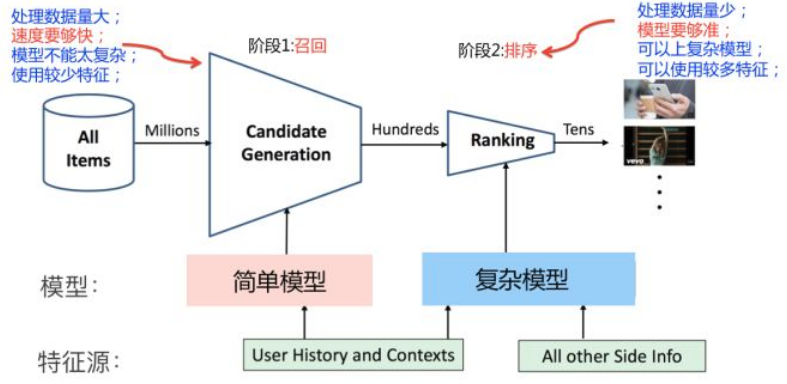
\includegraphics[width=4.8in,height=2.4in]{recsys}
\caption{推荐系统的两个模块}
\end{figure}

在介绍具体内容之前,\textbf{一起思考下面几个问题}:
\begin{enumerate}
\item{多路召回有什么优势?有什么缺点?}
\item{单路召回行不行?能不能用一个统一的模型来将多路召回改成单路召回?}
\item{能不能将召回阶段与排序阶段整合起来?有什么困难、不同?}
\item{多路召回如何选择K值?能否端到端优化?}
\item{不使用FM or DeepFM,直接使用DNN行不行?}
\end{enumerate}


FM \cite{DBLP:conf/icdm/Rendle10} 主要被用来处理高稀疏的特征。有类似LR的线性的计算复杂度。 在实际应用中常用来做排序。

\paragraph{FM模型} 假设 $x \in R^{n}$, 待计算的模型参数 $ w_{0} \in R, \textbf{w} \in R^{n}, \textbf{V} \in R^{n \times k}$.
$$\widehat{y}= w_{0}+\sum_{i=1}^{n}w_{i}x_{i}+\sum_{i=1}^{n}\sum_{j=i+1}^{n}\langle \textbf{v}_{i} ,\textbf{v}_{j} \rangle x_{i}x_{j}$$
where 
$$\langle \textbf{v}_{i} ,\textbf{v}_{j} \rangle =\sum_{m=1}^{k}v_{i,m} \cdot v_{j,m}$$

\paragraph{数学变换} 原问题的复杂度是$O(kn^{2})$. 通过一些数学变换可以优化到线性的复杂度 $O(kn)$. 达到了和LR接近的性能。
\begin{align*}
\sum_{i=1}^{n}\sum_{j=i+1}^{n}\langle \textbf{v}_{i} ,\textbf{v}_{j} \rangle x_{i}x_{j}
&= \frac{1}{2} \sum_{i=1}^{n}\sum_{j=1}^{n}\langle \textbf{v}_{i} ,\textbf{v}_{j} \rangle x_{i}x_{j} -\frac{1}{2}\sum_{i=1}^{n}\langle \textbf{v}_{i} ,\textbf{v}_{i} \rangle x_{i}x_{i} \\
&= \frac{1}{2}\sum_{m=1}^{k}\left( \left(\sum_{i=1}^{n}v_{i,m}x_{i}\right)^{2} -\sum_{i=1}^{n}v_{i,m}^{2}x_{i}^{2} \right)
\end{align*}

*哪来的$\frac{1}{2}$?

\section{LR、SVM、FM}
LR的特点: 模型简单,容易解释,规模弹性,人工构造or组合特征,学习一阶特征权重.
$$\widehat{y}=\sigma(w^{T}x)$$

SVM我们分两种来讨论:

线性核(linear kernel) SVM: $K(x,z)=1+<x,z>$。这里等价于d=1的FM
$$\phi(x)=(1,x_{1},...,x_{n})$$
$$\widehat{y}=w_{0}+\sum_{i}^{n}w_{i}x_{i}$$

多项式核 (polynomial kernel) SVM: $K(x,z)=(1+<x,z>)^{d}$, d=2时
$$\phi(x)=(1,\sqrt{2}x_{1},...,\sqrt{2}x_{n},x_{1}^2,...,x_{n}^2,\sqrt{2}x_{1}x_{2},...,\sqrt{2}x_{n-1}x_{n})$$
多项式SVM可以写成:
$$\widehat{y}= w_{0}+\sqrt{2}\sum_{i=1}^{n}w_{i}x_{i}+\sum_{i=1}^{n}w_{i}^{2}x_{i}^{2}+\sqrt{2} \sum_{i=1}^{n}\sum_{j=i+1}^{n} w_{i,j}^{2} x_{i}x_{j}$$
\noindent
\textbf{多项式SVM同样是二阶特征,跟FM比差在哪?}

要学习到一个足够可靠的$w_{i,j}$, 需要足够的$(i,j)$ case。 只要用户i 或者商品j 有一个为0, 就没有办法学习$w_{i,j}$。 如果数据非常稀疏,那么就意味着没有足够的case来学习$w_{i,j}$。

\begin{itemize}
\item SVM需要数据相对稠密,$(i,j)$之间交互要足够多。
\item SVM学习常需要转化成对偶形式,FM可以直接求解
\end{itemize}

对于FM来说,它可以通过低维向量间的相似性去估计$w_{i,j}$。哪怕$w_{i,j}$没有出现过。

举个例子来说,比如小A和小B都买了商品M,小B还买了商品N, 那么FM能够学习到:
$$<V_{A},V_{M}> \approx <V_{B},V_{M}>$$
$$<V_{B},V_{M}> \approx <V_{B},V_{N}>$$
$V_{A}$与$V_{B}$近似。 $V_{M}$与$V_{N}$近似。那么 $<V_{A},V_{N}>$的概率也应该很高。而对于SVM,信息是相互独立的,没有类似的范化能力。

\section{Matrix Factorization(MF)}
Matrix Factorization 矩阵分解的核心思想是通过两个低维小矩阵的乘积计算,来模拟真实用户点击或评分产生的大的协同信息稀疏矩阵,本质上是编码了用户和物品协同信息的降维模型。

\noindent
\textbf{和FM有什么不一样?}

MF可以被认为是只有User ID 和Item ID这两个特征的FM模型,MF将这两类特征通过矩阵分解,学习到user 和item 的embeddings. 而FM可以看作是扩展的MF, 可以加入更多的side info. 

MF类的模型不能引入其他信息(只考虑ID),明显不足够完备。这也是为何矩阵分解类的方法很少看到在Ranking阶段使用,通常是作为一路召回形式存在的原因。

\section{Field-aware Factorization Machines (FFM)}
FFM \cite{DBLP:conf/recsys/JuanZCL16} 主要是针对不同特征,细分到不同的field再学习一个独立的embedding.
$$\phi_{FFM}(\textbf{w},\textbf{x})=\sum_{i=1}^{n} \sum_{j=i+1}^{n}(\textbf{w}_{i,f_{j}},\textbf{w}_{j,f_{i}})\textbf{x}_{i} \textbf{x}_{j}$$

\begin{figure}[H]
\centering
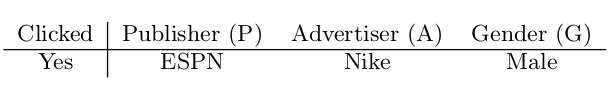
\includegraphics[width=4in,height=0.6in]{ffm1}
\caption{FFM 例子}
\end{figure}
\noindent
对于之前的FM来说:
$$\phi_{FM}(w,x)=w_{ESPN}\cdot w_{Nike}+w_{ESPN}\cdot w_{Male}+w_{Nike}\cdot w_{Male}$$
FM中不同的field (广告 or 性别),特征$w_{ESPN}$其实用的都是同一个向量。

FFM这些向量做了更细致的特征表达,对于每一个不同的field,都学习一个向量(Field-aware)。
$$\phi_{FFM}(w,x)=w_{ESPN,A}\cdot w_{Nike,P}+w_{ESPN,G}\cdot w_{Male,P}+w_{Nike,G}\cdot w_{Male,A}$$

假设一共有n个field,每一个特征都要训练n-1个向量。
在FM中,我们可以通过优化,把计算量降低到$O(kn)$。 而FFM无法做类似的优化,FFM的模型参数量是(n-1)*k *n, 计算的复杂度是$O(kn^{2})$. 带来的影响就是计算缓慢+过拟合。

论文中也提到这一点,特别提出了在FFM的情况下, $k_{FFM} \ll k{FM}$

\section{DeepFM}
DeepFM\cite{DBLP:journals/corr/GuoTYLH17} 是一种结合深度学习DNN与FM的网络结构。

通常我们在整理特征时,常采用one-hot来进行编码,这样做在DNN中有什么问题?

在离散特征很稀疏时,常常向量维度比较大,concate到一起后,输入层的长度也会很大。比如输入层有100w的节点,通过FC layer之后变成500个节点。模型需要计算5亿个参数,这样做是不可行的。如何解决呢? 结合分治的思想,先把每一个field都由稀疏向量转为稠密。也就是DeepFM中的Dense embeddings.

研究表明,单纯的MLP表达特征组合的能力很弱,我们希望能够把低阶的特征单独建模。也就是并行的融合高阶与低阶的特征。像Deep \& wide 中就采用了LR与DNN的组合,Wide 部分的LR以手工特征为输入。 DeepFM到这里也就几乎呼之欲出了: 把LR模块替换成FM,就是DeepFM模型。
$$\widehat{y}=\sigma(y_{FM}+y_{DNN})$$
$$y_{FM}=<w,x>+\sum_{i=1}^{n}\sum_{j=i+1}^{n}\langle \textbf{v}_{i} ,\textbf{v}_{j} \rangle x_{i}x_{j}$$


\begin{figure}[H]
\centering
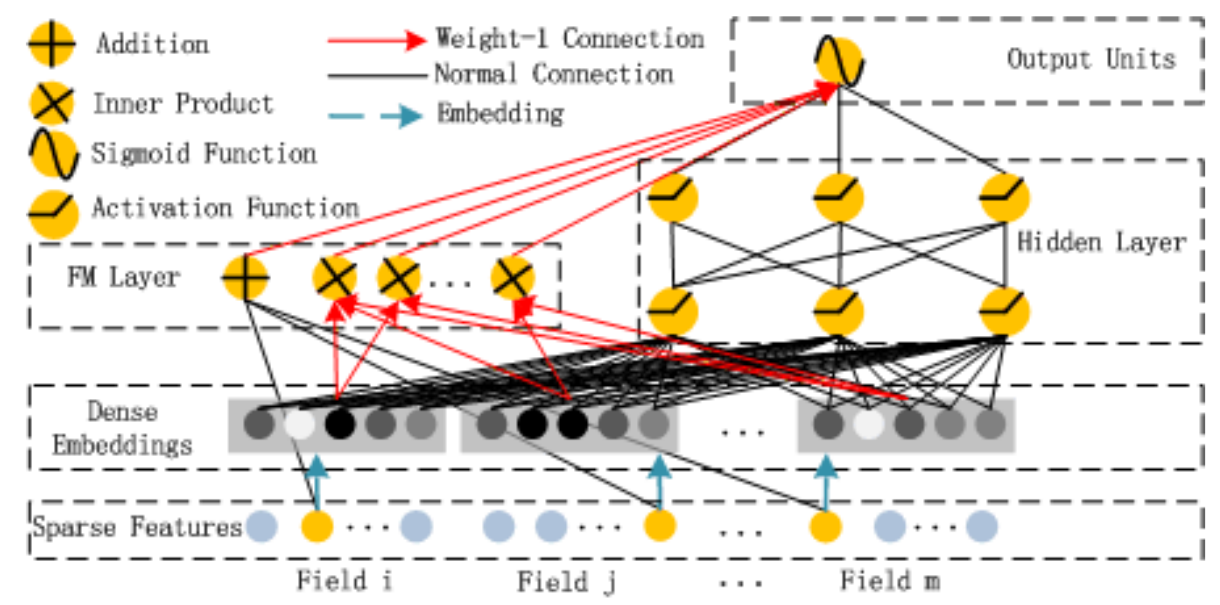
\includegraphics[width=4in,height=2in]{deepfm}
\caption{DeepFM 网络结构}
\end{figure}

DeepFM模型的特点:
\begin{itemize}
\item field 间各自embeddings
\item FM和DNN共享embeddings (为什么要这么做?)
\begin{itemize}
\item embeddings学习了高阶与低阶的特征交叉
\item 不再需要特征工程
\end{itemize}
\item 虽然不同field长度不同,但是embedding的长度是一样大的

\end{itemize}


\section{Answers ?}
\begin{enumerate}
\item \textbf{ 多路召回有什么优势?有什么缺点?}

\textbf{多路召回的缺点}:
\begin{itemize}
\item 不同策略召回的item打分不能统一比较,所以需要靠ranking模型来进行打分。
\item 多路召回的另一个问题就是,每一路应该选多少候选集?也就是K值的选择。每一路的K值其实是超参数,线上需要不断调整,其实我们并不知道最优的k的组合是什么。理解的情况,每个用户对不同路的召回兴趣是不同的,所以不同路的召回应该有不同的K值。
\item 在排序ranking部分也有可能产生一些问题,新增的召回策略有可能没有把相对应的特征加到ranking中,导致新增召回路看上去没什么用,因为即使你找回来了,而且用户真的可能点击,但是在排序阶段死活排不上去。
\end{itemize}

\textbf{多路召回的优点}:
\begin{itemize}
\item 上线新召回算法比较灵活
\item 不同路召回之间没有耦合关系,上线一个召回不会影响其他模型
\end{itemize}

\item \textbf{ 单路召回行不行?能不能用一个统一的模型来将多路召回改成单路召回?}

可以。 FM构造一个单路召回的模型
$$\widehat{y}=FM(User,Item,Context)$$

\begin{figure}[H]
\centering
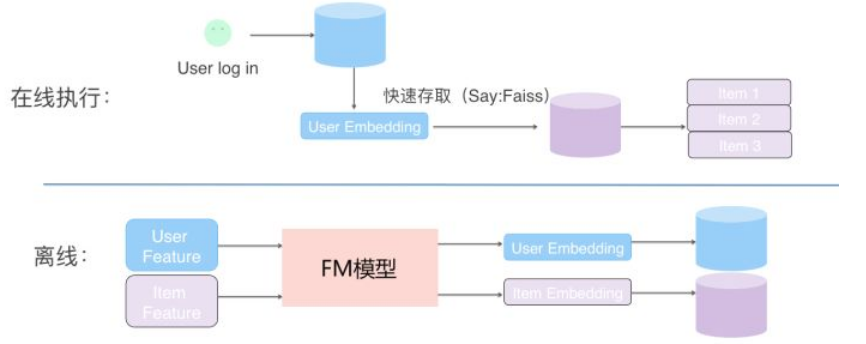
\includegraphics[width=4.8in,height=2in]{fm1}
\caption{最简单的FM模型,暂不考虑context}
\end{figure}
加入一阶特征trick: 在原始的FM/FFM中,是有一阶特征的(LR部分),如何在召回时也加入这部分 ?
\begin{figure}[H]
\centering
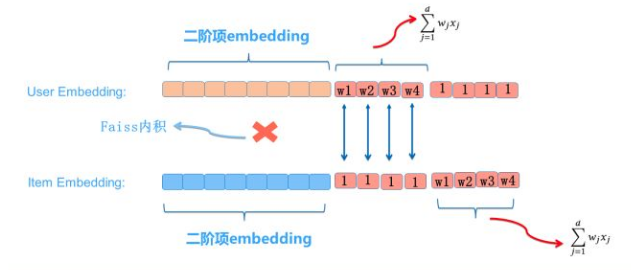
\includegraphics[width=4.5in,height=2in]{fm2}
\caption{user特征累加,对应item位置置1}
\end{figure}

结合context: 一种思路可以是计算context特征的sum average,然后通过$U+C$去召回出Item,根据$<U,C>$进行Item排序。
\item \textbf{能不能将召回阶段与排序阶段整合起来?有什么困难、不同?}

要将这两块整合,主要考虑两个方面:1、速度(海量数据的查询,例如 similiarity search topk embeddings的速度)。2、精度(没有了粗排之后,精度还能否有保障?)

如果是在排序阶段使用FM/FFM或者其他模型,因为此时用户已知,要排序的具体是哪篇文章也知道,都是少量数据,此时模型的任务是要判断用户是否对某篇文章感兴趣,所以用户特征和物料特征可以同时作为模型的输入。

而如果是在召回阶段使用FM/FFM模型,user的信息是有的,但是item的信息往往是千万量级的,要求模型在海量数据中找到那一小批用户感兴趣的item出来,而且要保证速度。

\item \textbf{不使用FM or DeepFM,直接使用DNN行不行?}

只使用DNN, 对于低阶的组合特征,比较难以学习到的低阶特征。而对于CTR领域, 低阶特征是非常重要的。这一思路在后来的DCN网络结构中也有体现。最原始的$x_{0}$一直都作为每一层的直接输入。
\end{enumerate}

\bibliographystyle{plain}
\bibliography{ref}

\end{CJK*}
\end{document}

























